\documentclass[10pt,twocolumn]{article}

% use the oxycomps style file
\usepackage{oxycomps}

% usage: \fixme[comments describing issue]{text to be fixed}
% define \fixme as not doing anything special
\newcommand{\fixme}[2][]{#2}
% overwrite it so it shows up as red
\renewcommand{\fixme}[2][]{\textcolor{red}{#2}}
% overwrite it again so related text shows as footnotes
%\renewcommand{\fixme}[2][]{\textcolor{red}{#2\footnote{#1}}}

% read references.bib for the bibtex data
\bibliography{references}

% include metadata in the generated pdf file
\pdfinfo{
    /Title (Using Markov Chains for Music Generation)
    /Author (Will Baron)
}

% set the title and author information
\title{Using Markov Chains for Music Generation}
\author{Will Baron}
\affiliation{Occidental College}
\email{wbaron@oxy.edu}

\begin{document}

\maketitle

\section{Introduction}

Music and computer science are incredibly similar. On the surface, it seems like music is very "right brain" dominated, meaning it requires a lot of creativity, imagination, and feeling. Computer science on the other hand appears very "left brain", using logic and rigid guidelines to achieve a desired result. Through my years of study in both fields, I've found that both areas have much more overlap than people think. There are lots of binary metrics that explain the feeling behind music, for example a note's relation to the key center can often be used to justify its unique tension that evokes a certain feeling. Additionally, computer science requires a great deal of creativity to come up with efficient solutions to solve problems and innovate across the ever expanding field.\newline

My project aims to synthesize the two fields and use the under-rated creativity of computer science to replicate the overlooked guidelines of music. I've made a music creation tool, the primary purpose of which is to assist songwriters in writing music over a given chord progression.

\section{Problem Context}

Writing music is tough. If you don't constantly work to try out new things, you can get stuck writing in the same style and using similar sounding sequences. As a recreational musician, my solos sound pretty similar song to song and I've been using the same musical toolbox for a while. My project introduces new musical ideas that I can add to my musical toolbox and spice up my playing.

\section{Technical Background}

\subsection{Software}
        For my project, I used the visual programming language Max/MSP/Jitter (Max). Max is mainly used for developing interactive music performances, but it lends itself very well to the goals of my project. Max is an object oriented visual programming languages that operates through patches\cite{Max}. You instantiate various objects and connect them to make things happen. The simplistic nature of the language is very quick to learn but has immense potential.
        
    \subsection{Markov Chains}
        Markov chains are systems that tell you the probability of transitioning between states. You can record the number of transitions between states and calculate the probabilities in order to recreate a set of transitions that is close to the original data\cite{Markov}. For my project, each state in the various Markov chains is related to some musical concept. One chain is note choices, or the transition table from one note to another. Each state is a note and more common transitions from one note to another is reproduced more. Another Markov chain holds the duration of notes. If there are lots of parts where notes are played really fast, the probability of a note being shorter in duration transitioning to another note that is shorter in duration will be very high. Using these chains in addition to some others, music is made that is inspired from the training data.\newline
        
        The training data is the music from which the Markov chains actually record the transitions. Using music from different artists, I've created multiple sets of Markov chains, each with different probabilities based on the artists music. For example, one of the artists I've chosen is Miles Davis. I've fed a copy of my Markov chains songs from Miles Davis to train them on his style. The Markov chains record his note transitions and rhythm transitions so they can create music using his musical habits.\newline
        
        I chose to use Markov chains for my project because of the simplicity of the implementation and how good it is at working with melodies. Since my project revolves around single note melodies or solos, Markov chains are a perfect data structure to use.

    \subsection{MIDI Files}
        My Markov chains take in MIDI files as their inputs. MIDI files are a universal file format that can be shared and interpreted across a wide variety of software programs. They consist of a series of instructions that tell the software what note to turn on, when to turn it on, and with what velocity to turn it on with. A separate instruction will contain a note off message. MIDI files contain velocity information which replaces volume information. Along with being louder, a high velocity note, depending on the software, will have a different, more aggressive sound. A low velocity note will be quieter and usually softer. One of my Markov chains tracks transitions between velocity values to account for different musical dynamics. I chose MIDI files because of their extreme versatility and wide availability online. There are numerous large MIDI file libraries with an infinite supply of music files which are very easy to edit for my needs.
        
    \subsection{Music Theory}
        To understand my project, a very basic knowledge of music theory is required. Our western style of music is based off of 12 different notes. The distance between one of these 12 notes and its neighboring note is called a half step. A whole step is two half steps. You can create smaller groups of these notes called scales that you construct melodies, chords, and entire songs out of. A scale is a collection of usually 8 notes and in many cases it is either major or minor. The only difference between a major and a minor scale is the distance between the notes. For example, the distance between the seventh and eighth scale degree in a major scale is a half step while in a minor scale it is a whole step. These different intervals work to create different moods and feelings associated with different scales.\newline 
        
        If you wanted to make a chord, you would take the first, third, and fifth scale degrees and play them at the same time. Similarly to scales, the only difference between a major and minor chord are the intervals between the notes. To make a major chord, you use a major scale for your three scale degrees and for a minor chord you use a minor scale. If a song is in the key of C Major for example, you take the interval template for a major scale and you start on the note C. This restricts you to the following notes: C, D, E, F, G, A, B, C. You use these notes to create all your chords and melodies. If you use other notes from outside the previous eight, you've used what are called non-diatonic chords or notes. \newline
        
        Non-diatonic chords and notes can create a lot of tension since they are less commonly used, so your ears perk up when you hear them. For a solo, you usually stay within the eight notes from your key, only tastefully borrowing non-diatonic notes. Depending on what chord you are playing at the time, the impact of your note choice is furthered. Even though you are in the key of C, and B is in the key of C, if you are playing a B over a C major chord, it may sound especially dissonant because of the close proximity of the notes B and C. Since they are so close to each other, they can sound "bad" unless used in the right context. If used in the right context, the dissonance is quite interesting and satisfying to hear. \newline
        
        Initially I thought about restricting the notes my model could output to sound more diatonic, or "good" but then I realized that would go against the goals of my project. I want my model to produce interesting musical ideas, which I won't get as many of if I restrict it to only notes within the scale implied by the chord progression. This has led to my model sometimes making music that doesn't sound very good, but leads to creative and original new music.
        
\section{Prior Work}
    Filippo Carnovalini and Antonio Roda cover a great introduction to music generation systems in an article aptly titled \textit{Computational Creativity and Music Generation Systems: An Introduction to the State of the Art}\cite{Markov}. They cover seven of the main methods for music generation, one being Markov chains. In particular, they detail how Markov chains are well suited for melody generation in the case of the chains only containing pitch information. Since the Markov chains can only hold one type of state, the paper suggests using multiple in tandem like I plan to do.\newline
    
    \textit{Generating Guitar Solos by Integer Programming} by Nailson Cunha, Anand Subramanian, and Dorien Herremans take a different approach by quantifying the transition cost of playing one guitar lick after another and using this cost matrix to calculate the most efficient sequence of licks that fits into a 12-bar blues\cite{Guitar}. Additionally, both papers use a similar method of analysis. Both include a form of surveying the audience for their opinions. In \textit{Generating Guitar Solos by Integer Programming}, a study was conducted in which the participants selected between a random pattern of licks or an optimized pattern of licks based on enjoyment. This type of evaluation metric is something I plan to use as well. \newline
    
    MuseNet and Magenta are two of the most well known musical generation projects. MuseNet is a model that generates music compositions with different styles and instruments. The software behind MuseNet is very well documented with tutorials, libraries, and guides on using capabilities of the program. The program uses a technology called sparse transformers which is a type of sequence model that is very efficient in terms of memory usage and training speed\cite{SparceTransformers}. Further research on this topic specifically is necessary to determine the feasibility that I use it myself or not\cite{MuseNet}. Magenta is an open source project from Google that offers tools for making music with machine learning. On their website are many datasets they used including NSynth which contains over 300,000 musical notes with distinct timbres. If I decide to work with timbres this dataset will prove very useful. Additionally, the Bach Doodle Dataset features 21.6 million harmonizations and melodies\cite{Magenta}.


\section{Methods}
    Initially, I wanted to use a different method to go about my project. I wanted to use TensorFlow to create a Recursive Neural Network that learned from the music of different artists to create new music. I wanted to write a neural network because I thought it would be a good challenge and I've always been interested in how they work. I based my idea off of how Magenta\cite{Magenta} uses user input to extrapolate and create new music, and I wanted to go that route. Magenta is a TensorFlow project as well, which drew me closer toward using it for my project. I tried to get TensorFlow to work on my system for about two weeks before I gave up due to numerous hardware conflicts. I used alternate conda environments to install different software packages to get around the native conflict TensorFlow has with the M1 chip. This got me close, but after weeks of trying to resolve package dependency issues based off of hardware and software conflicts and not making any progress, I gave up. I tried a similar approach with PyTorch, but I ran into many similar issues. My next idea was to write a neural network myself, but given that I had lost weeks of time, I did not think that was realistic. I opted for Markov chains after that since I had worked with them before and I knew I could achieve my goals.\newline

    While researching Markov chains, I came across a wildly helpful YouTube tutorial that helped me get started implementing Markov chains in Max\cite{Vid1}\cite{Vid2}\cite{Vid3}. After I had implemented the ability to create music in the style of different people, I began working on the chord progression implementation. After I had figured out the chord progression playback, I began gathering data. I used various online MIDI file libraries\cite{Kaggle}\cite{BushGrafts}\cite{FreeMidi} to chose three pieces for each artist. I trimmed down the MIDI files which contained a lot of extra music besides the solo artist I was looking for by loading them into Logic Pro, a music editing software, and deleted all the extra information. I then exported again for my final data.\newline
    
    For the actual implementation of my project, Max has a great object for Markov chains that is very intuitive to use. 
    \begin{figure}[h]
    \centering
    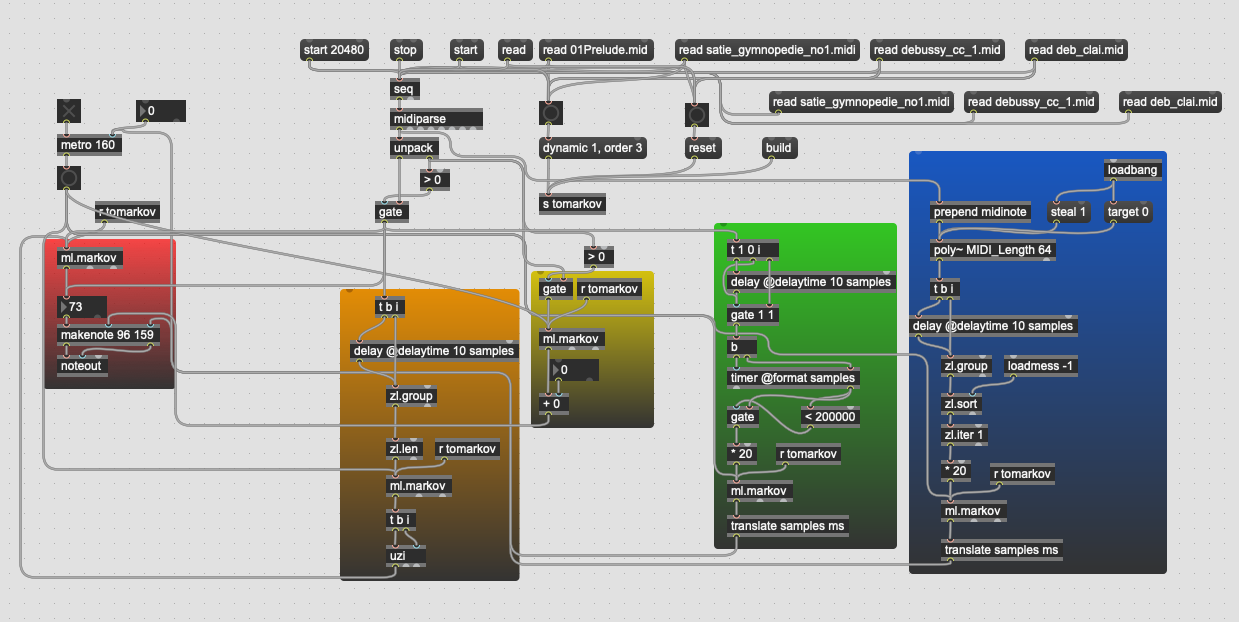
\includegraphics[width=1\linewidth]{final.png}
    \caption{
        My main sub patch that contains Markov chains.
    }
    \label{fig:second}
    \end{figure}
    The note choice Markov chain is shown in the red panel. The orange panel delays the note input shortly to collect the number of notes being played at once in the case of a chord. This then tells the first Markov chain to play that many notes at once to account for chords. The yellow panel creates a Markov chain for velocity information which is relayed to the output. The green panel starts and stops a timer when notes are turned on/off. This Markov chain holds note length information which tells the metro object when to tell the original ml.markov object to play the next note. The blue panel accounts for the duration of multiple notes. The notes that are on at any given time are sorted by longest elapsed length first and sent to a ml.markov object. This Markov chain directly influences the duration of the next note in the makenote objects duration inlet. As you can see, a wide variety of musical parameters are accounted for by only a few Markov chains.\newline

    The chords are sent to a patch where the notes to play are figured out. Based off of the root note and the quality (maj/min) of the chord, the patch does some quick addition to calculate the midi note value of the third and the fifth of the chord. The root, the third, and the fifth are combined and sent out of the patch to be played. A separate patch receives all the chord information and by using a metronome that outputs a steady signal at consistent time intervals, plays each chord four times before cycling to the next one. \newline

    For my project, I fed the Markov chains midi samples from different artists to populate the chains. Different artists have vastly different styles that can be reproduced by populating my Markov chains with data from their music.
    \begin{figure}[h]
        \centering
        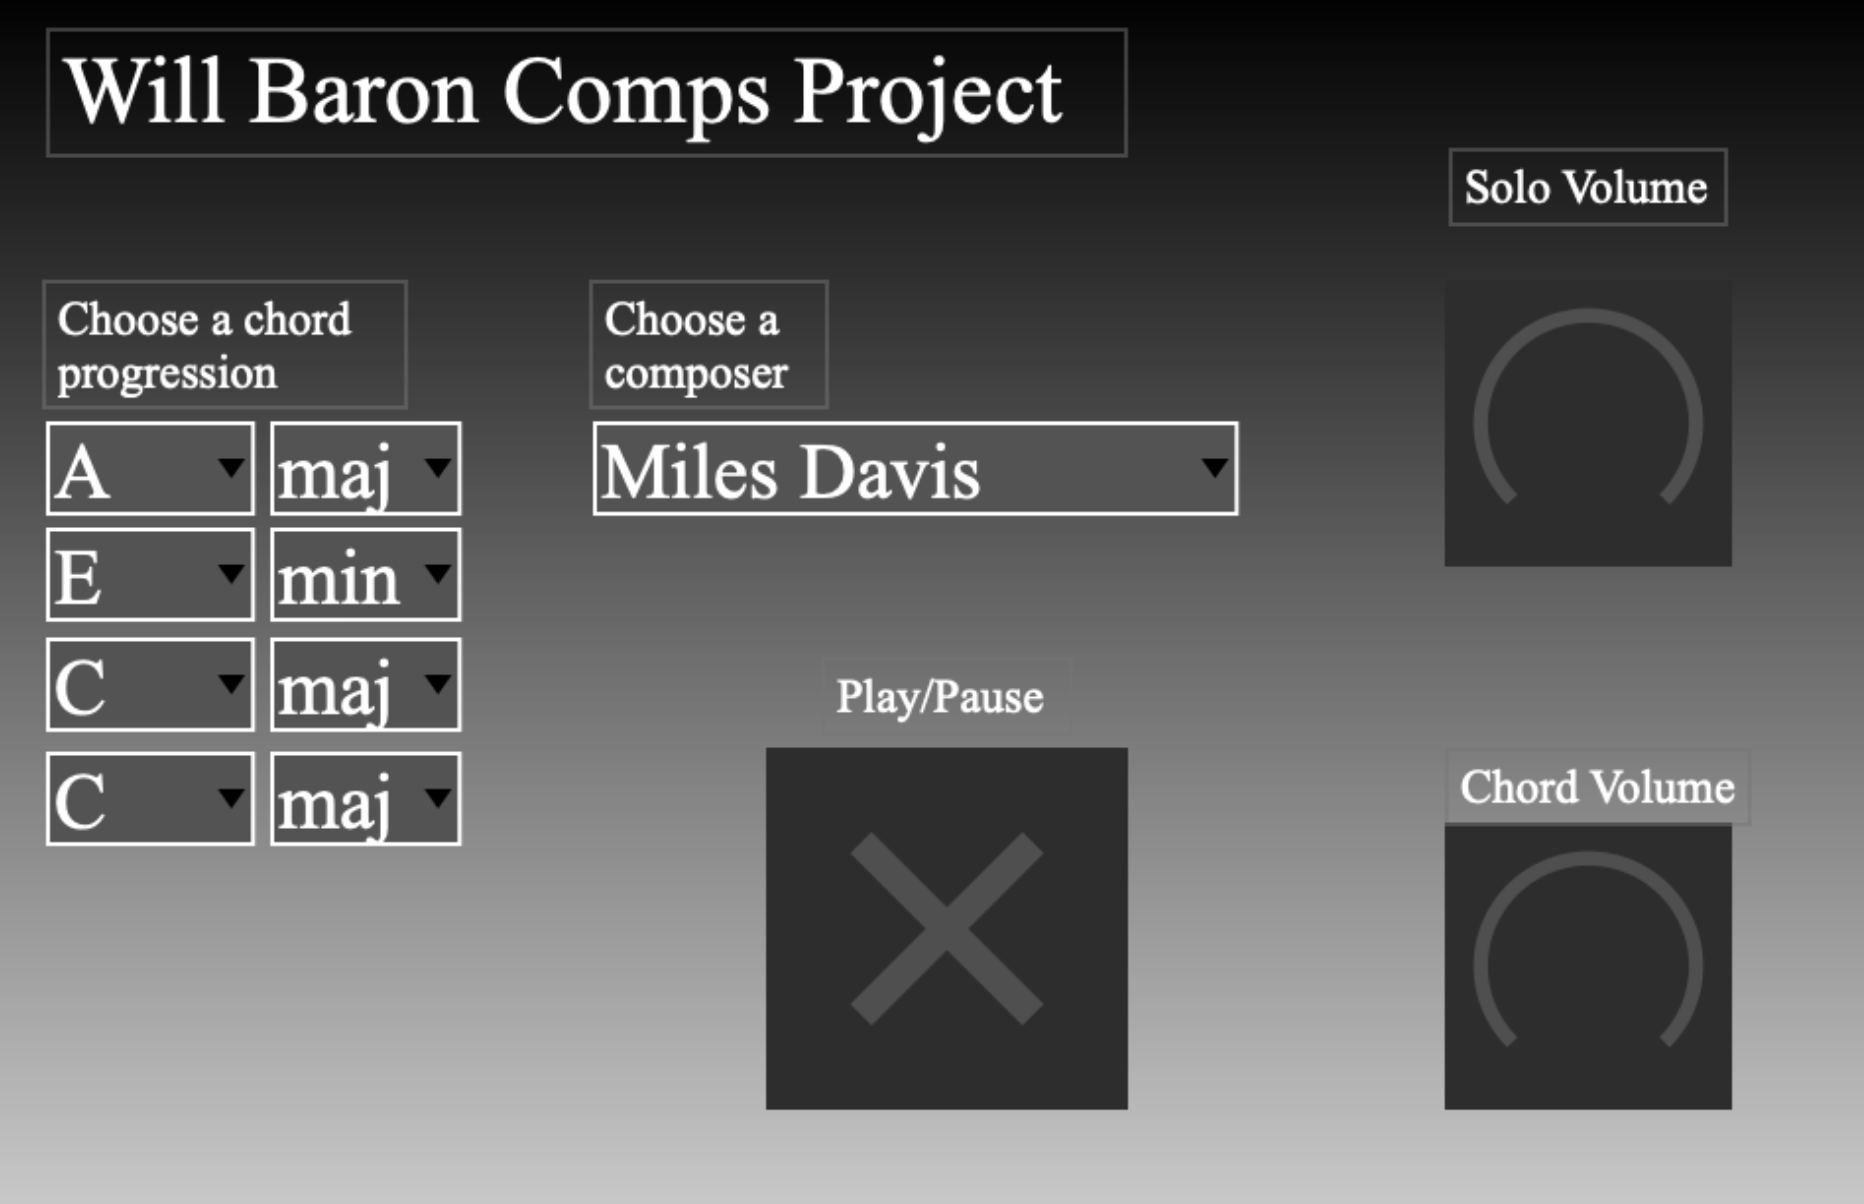
\includegraphics[width=.95\linewidth]{ui.png}
        \caption{
            My project UI.
        }
        \label{fig2}
    \end{figure}
    In the UI in Figure 2, the user inputs a chord progression with the set of menus in the top left, selects a composer with the middle menu and sets the volume with the dials on the right. The patch takes that chord info and turns it into a four chord loop. The composer selection determines the style in which my model plays since the different Markov chains will have different transitions based off the different composers.

\section{Evaluation Metrics}
    
    The previously mentioned study by Nailson dos Santos Cunha gauged the success of their work by a survey in which the participants selected between a random pattern of licks or an optimized pattern of licks based on enjoyment. Since the participants chose the optimized pattern significantly more, they deemed their project a success. I wrote a solo over a chord progression, then I enhanced it with various musical sequences from my project. I presented users with both solos and asked ten of my peers which one they enjoyed more. In the mp3 titled "Comps Evaluation" in the GitHub, the first 57 seconds are my original solo, followed by a sample output of my program. Each time my program plays a musical phrase that I like, I play it on guitar immediately after. Following the output of my program, from  2:23 until the end of the mp3 is my enhanced solo, incorporating the musical phrases I liked from the output of my program.\newline

    An alternate evaluation I considered comes from a paper by Li-Chia Yang and Alexander Lerch titled "On the Evaluation of Generative Models in Music"\cite{Evaluation}. This paper details a way to objectively evaluate music based on various metrics such as:
    \begin{itemize}
        \item Pitch count - the number of different pitches within a sample
        \item Pitch range - the range between the highest and lowest pitch in a sample
        \item Average pitch interval - the average value of the interval between two consecutive pitches
        \item Note count - the number of used notes
        \item Average inter-onset-interval - the average time between two consecutive notes
    \end{itemize}
    The model containing these metrics can be trained using a certain genre of music, such as folk or jazz, and can generate these results based on the input data. The music created by generative models can then also be evaluated using these metrics and the two sets of metrics can be compared. In my project, I could have trained the model with the MIDI files I provided to my Markov chains and analysed my generated music to get my sets of metrics to compare. Unfortunately, I could not get the model provided in this paper to run on my computer, preventing me from using this resource. 

\section{Evaluation Results}
    Upon surveying ten of my peers, six people enjoyed my original solo more while four people enjoyed my enhanced solo more. Additionally, using my program to enhance my solo gave me interesting musical ideas that I will discuss in the next section

\section{Discussion}
    There are several topics I will cover in this section:
    \begin{itemize}
        \item Was my project successful based on the survey?
        \item Was my project successful based on my own user experience?
        \item Could my project have benefited from a more objective evaluation system?
    \end{itemize}
    \subsection{Survey Success}
        Based on my survey, my project was not successful. 4/10 people enjoyed the enhanced solo which is an underwhelming success rate. This implies my project was not successful, but was a survey the best evaluation for my type of goal? My original goal was to create a tool that assists musicians in writing music, not to necessarily write better music. If my model gave someone new ideas, or to go back to my original analogy, gave someone new tools for their toolbox, it was successful. Upon reflection, my survey does not accurately capture the goals of my project. If anything, my survey serves as validation that my original solo was more interesting, even though I didn't use anything new or interesting to me.

    \subsection{User Experience Success}
        My user experience was quite interesting. Upon listening to the output of my model, I was worried that it was going to be unusable garbage. Some of it was not usable, but every so often as you can hear in the mp3, there are distinct musical phrases that play that provide exactly what I wanted when I set out to make a musical tool. Hearing these phrases, transcribing them on my guitar, and using them in a solo, gave me many new melodic and rhythmic ideas. The last phrase for example uses a G minor scale over a chord progression in G major. This idea is not revolutionary in the field of music theory, but it was a sound I was not used to playing. This forced me outside my comfort zone and it made me realize how easy it was to achieve a new sound. Now I have this new musical tool in my toolbox, which was the original goal. In this sense, my project was successful. A survey that was more oriented toward this process would have much more accurately represented my project. I could have sent my project out to some musicians and gotten their opinions on their user experiences and if they would actually use it or not. This would have given me more of an idea of what I need to make better in my project and if it actually helped people write music.

    \subsection{Objective Evaluation System}
        All of my previous evaluation systems have relied on user experience and intangible data. In order to collect empirical data, I had originally suggested using the analysis tool from "On the Evaluation of Generative Models in Music"\cite{Evaluation}. This tool, like my survey, may not accurately represent the goals of my project. I don't necessarily want to compare my work to the music I used to train it. If I wanted to hear the musical ideas of Miles Davis, I would listen to his music. Using his work as an inspiration for new ideas is more of what I want to achieve. Using the evaluation tool from the aforementioned paper would result in music with a higher score sounding more like the original, which is not what I want. 

\section{Ethical Considerations}
    \subsection{AI Copyright Issues}
        If I were to deem the music created by my project my own, what legal ramifications does that pose? Especially since I trained my model using preexisting music, what happens if I get sued by Miles Davis's legal team for replicating his work? As of now, the law doesn't account for music created by non-humans, but if I only fed my model works by Miles Davis, and the output sounded a lot like a Miles Davis song, there might be some grounds for Miles Davis's legal team to take action\cite{Law}. Additionally, if I put out this music and claim myself as the songwriter, am I really the songwriter? The big issue I want to avoid is people thinking I stole music, which could actually happen if I use a famous phrase that I got from my project in my own music. If interpolation wasn't such a big part of jazz culture, I might be in trouble, but since jazz musicians quote each other all the time, it is not such a big deal. In a paper by Kara Smith, she notes how, "In the spirit of interpretation, when a musician cites compositions by great jazz musicians of earlier periods, it is a way of passing things along and it exemplifies where they themselves have been. It also shows the respect that the musician has for all of the terrific motives and lines that came out of that style of music."\cite{Interpolation} If I tried to market the music that the AI produces as my own, there might be some issues, but since I am only drawing inspiration from the music of my project, there is no problem. 
        
    \subsection{Lack of Disability Support}
        If someone cannot hear my project, they cannot enjoy my project. To solve this problem, an option would be integrating some sort of music scoring software to transcribe the output for people to read as they cannot listen. This requires people to be able to read music which reduces the population of people who can use my project significantly, and if someone cannot hear or read music, they cannot interact with my project at all. \newline
        
        Another option for the hearing impaired is experiencing music through vibration, however this requires technologies and mediums that I do not want to explore, and the population of people that would need it is too small to warrant exploration (hearing impaired and cannot read music). Addressing these ethical concerns would derail my project since I would have to focus on implementing the sensor technology, and while interesting, I do not have access to these sensors, and their use cases are so niche it would not be worth the implementation.\newline
        
        For those who are visually impaired, using the UI will prove difficult, however using any visual UI will prove difficult. The majority of products today use some form of visual UI for input. To address concerns in this category I would need to develop an alternate system of input using tactile responses or sound. The issues with implementing a tactile response system for inputs are the same as the issues with musical vibrations in the previous point, and the issues with creating an interface controlled by sound have a similar cost to reward ratio as the previous point. Solving these challenges creates more challenges for other people. If I create a UI based off of sound, then those who are hearing impaired are affected. If anyone falls under both categories, they simply cannot use my product. \newline
        
        Research from the University of Washington, Seattle reveals that in the past 26 year period, research on accessibility has been heavily focused on this category with 43.5\% of papers about blind/low vision disabilities \cite{Accessability}. Almost 37\% of papers were aimed at developing new technologies to increase accessibility. Implementing these new technologies is not feasible given the time frame.
    
    \subsection{Western Music Theory Based}
        If I pitch my project as being able to help musicians, but the chord interface only supports theory from the western sphere of musical influence, am I really providing a service to everyone? The music theory that we study and are familiar with comes from early classical music from Europe. Music theory is based off of composers such as Mozart, Beethoven, and Bach and their use of music melodically and rhythmically \cite{Neely}. The way they constructed their music is still regarded as "correct" and is how we are taught to do so to this day. This is how I grew up in music education, but it completely discounts music from the rest of the world. Many other styles of music don't even use the same notes we do. The way we organize our notes is called the 12-tone scale, but other cultures such as India, organize their octave into 22 parts and Turkish classical music has names for 53 tones\cite{Microtones}. The sounds from other parts of the world are completely different and sound foreign to those of us that grew up with curriculum based off European composers.`Additionally, new rhythmic ideas are found in various cultures from Africa which center largely around different types of drums. Drum circles are still integral parts of African culture and feature complex polyrhythms and time signatures.\cite{Poly} Polyrhythms are when two different rhythms are played at the same time. They can sound chaotic and sloppy to unfamiliar ears but when an entire culture is based off of them, they sound normal and are actually used to dance to despite their sometimes confusing sound. My project will use western music theory with western scales and rhythms that are only common in western music. Chord types that other musicians from different parts of the world want to use might not be possible which prevents them from using my project. There is always a risk in creating any type of content that someone might not like the result. This should not prevent you from creating the type of content you want to create as long as it doesn't put anyone in danger.

    \subsection{Requires Some Knowledge of Music Theory}
    The majority of people might not be able to create a diatonic chord progression, so a "Help" panel would have been useful for my project. This help section could have given a very simple guide on how to create a "good" chord progression and explain why random chord choices sound "bad". This help section could also have detailed the different artists and how they affect the style of the output.

\section{Future Work}
    If I were to continue this project I would add the help panel I mentioned in the previous section. Additionally, I would add support for different artists and expand my training data library. I would also add more chord voicing options, like maj7, min7, and dom7 to more align with the jazz genre and to be more versatile. Finally, I would export this into a standalone application that isn't tied to Max. Max is not as well known as some other programming languages and its main purpose is so niche that it isn't very well supported. This would make the distribution of my project much easier and people wouldn't have to register for a Max account or know how to use the language. 

\section{Conclusion}
    My goal was to help musicians write music by giving them a source of inspiration based on different artists work. While not represented in my results, I believe I achieved that through my own personal use. I've found new musical ideas that I can incorporate into my playing and I created a means to combine my passion for both music and computer science.
    
\printbibliography

\end{document}
